\chapter{Spektrale Methoden\label{chapter:klima}}
\lhead{Spektrale Methoden}
\begin{refsection}
\chapterauthor{Peter Nötzli}

\section{Einleitung
\label{klima:section:einleitung}}
\rhead{Einleitung}
\index{spektrale Methoden}

\begin{figure}
\centering
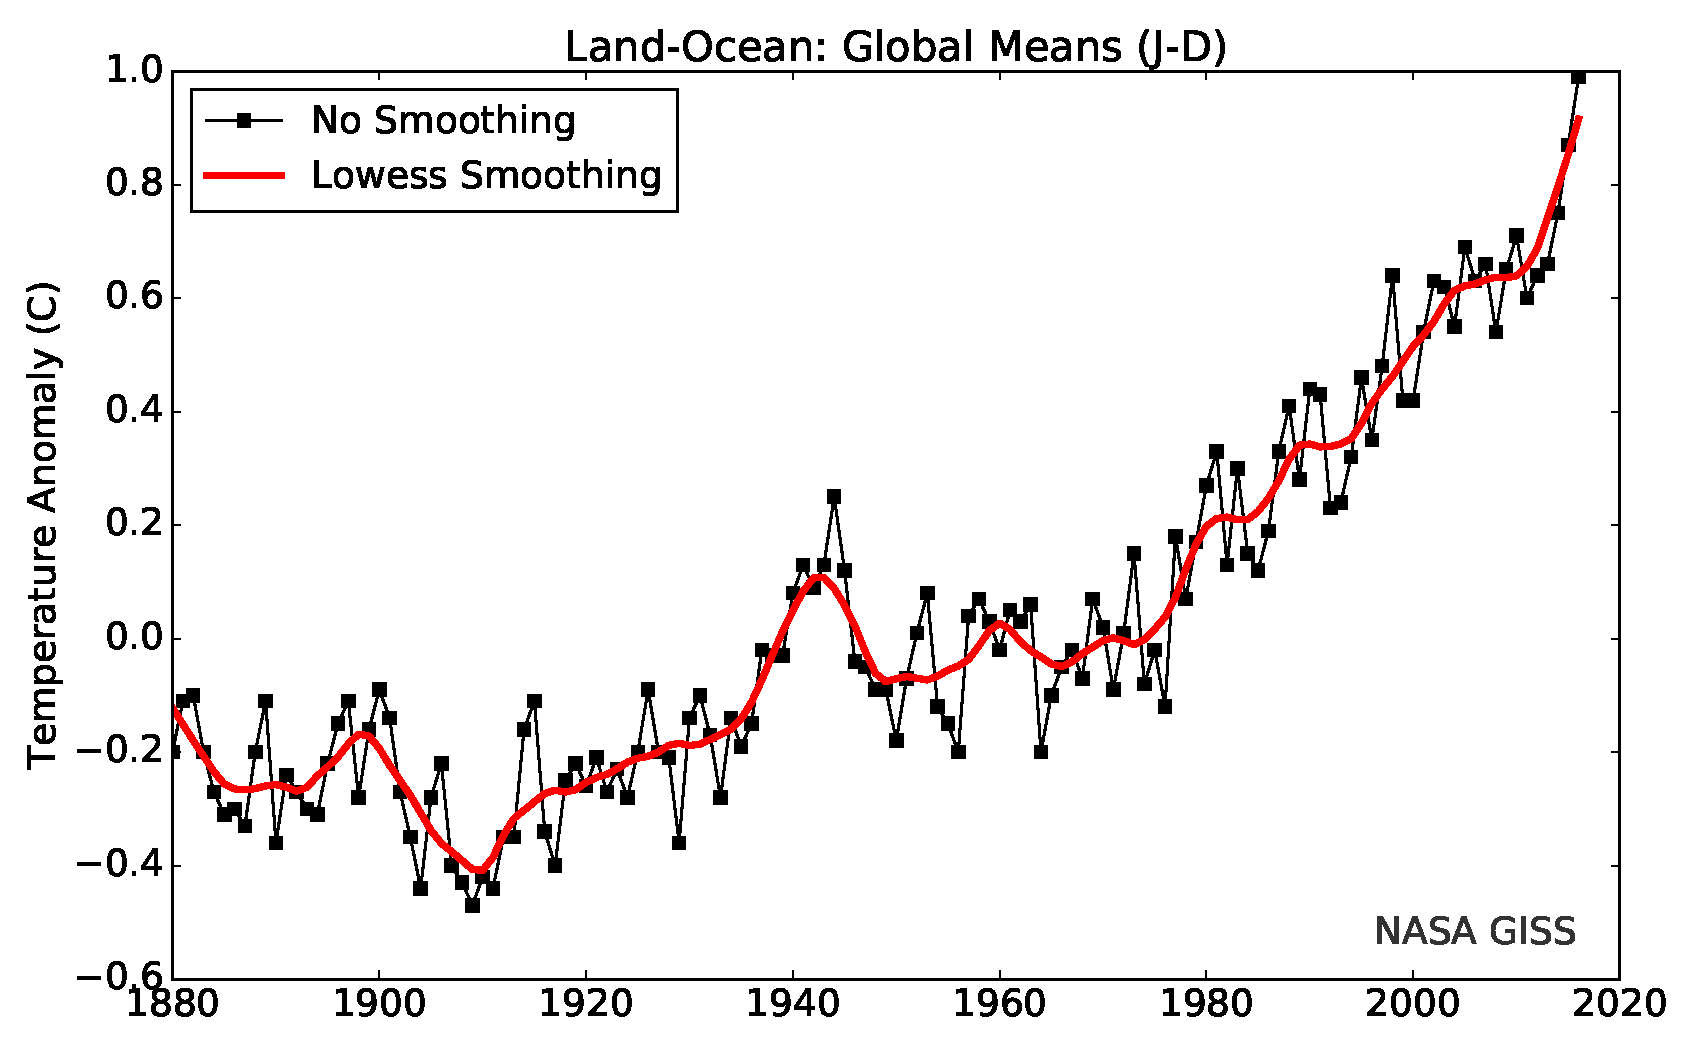
\includegraphics[width=0.9\textwidth]{klima/nasa_giss.pdf}
\caption{Grafik der globalen Jahresmitteltemperaturen seit 1880. \cite{klima:nasa}.
\label{klima:einleitung:nasa}}
\end{figure}

Die Klimaerwärmung\index{Klimaerwärmung} schreitet voran, gleichzeitig, oder gerade deswegen kommen in der Gesellschaft dazu immer mehr Fragen auf. Gibt es eine Klimaerwärmung? Wie entwickelt sich diese? Was bedeutet dies für uns? Betrifft es mich überhaupt?

Die erste und wohl einfachste Frage vorweg, ja es gibt die Klimaerwärmung. Dies ist deutlich zu erkennen wenn wir die globale Temperaturentwicklung seit 1880 bis heute betrachten (Abbildung~\ref{klima:einleitung:nasa}). Diese Frage ist deshalb einfach zu beantworten, da diese nach einer Entwicklung fragt welche bereits, oder zumindest teilweise, in der Vergangenheit liegt. Die Auswirkungen dieser Entwicklung und wie weit diese noch fortschreiten wird sind Dinge, welche in der Zukunft liegen. Möchte man Fragen zur zukünftigen Entwicklung beantworten bedingt dies eine Weiterführung der bereits bekannten Funktion. Obwohl eine Tendenz der Temperaturentwicklung erkennbar ist, kann aus dieser keine Aussage zur zukünftigen Temperaturentwicklung gemacht werden. Da wir dennoch gerne wissen wollen welche Einflüsse welche Auswirkungen haben und wir auch nicht warten möchten bis es bereits zu spät ist, müssen wir auf Klimamodelle zurückgreifen. Wie solch ein Klimamodell\index{Klimamodell} ausschauen könnte und wie es aufgebaut sein kann, soll in diesem Kapitel aufgezeigt werden.

\section{Geschichte der Numerischen Strömungsmechanik
\label{klima:section:geschichte}}
\rhead{Geschichte}
Die numerische Strömungsmechanik, heute auch als CFD bekannt (Computational Fluid Dynamics\index{Computational Fluid Dynamics (CFD)}) bezeichnet eine etablierte Methode, um verschiedenste Problemstellungen der Strömungsmechanik approximativ mit numerischen Modellen zu lösen. Die Validierung der Methoden erfolgt durch den Vergleich mit quantitativen Experimenten.

\subsection{Entstehung der Wettervorhersagen
\label{klima:subsection:wetter}}
\index{Wettervorhersagen}
Am Anfang war das Wetter. Dann kam der Mensch und wollte wissen, wie das Wetter in Zukunft sein wird. Dies aus verschiedensten Gründen so wollen wir heute gerne wissen, welches Wetter am Wochenende ist, damit wir bereits anfangs Woche einen Ausflug organisieren können.

Bedeutung hatten Wettervorhersagen, früher wie heute, so kann eine Wettervorhersage Wesentlichen Einfluss auf das Ernteglück haben. So entstanden schon früh sogenannte Bauernregeln, diese gingen meist davon aus, dass sich das Wetter aufgrund Wetterereignissen an bestimmten Tagen in eine gewisse Richtung entwickeln. Die Korrektheit solcher Aussagen sind wohl eher Zufälle als korrekte Vorhersagen, so sind es eher die ähnlichen Wetterverhältnisse der jeweiligen Jahreszeit welche solch eine Regel von Zeit zu Zeit als korrekt erscheinen lässt. Jedoch waren verschiedenste Naturphänomene bereits bekannt, als Beispiel die Silberdistel\index{Silberdistel}, auch als Wetterdistel\index{Wetterdistel} bekannt, welche ihre Blütenblätter bei erhöhter Luftfeuchtigkeit aufrollt und so vor nahendem Regen warnen kann.1660 erkannte Otto von Guericke erstmals den Zusammenhang zwischen abfallendem Luftdruck und dem Aufziehen eines Unwetters.

Anfangs des 19. Jahrhunderts entstanden in Europa die ersten Wetterstationen\index{Wetterstationen}, es waren jedoch noch keine Wettervorhersagen möglich. Der Grund dessen war die langsame Informationsweiterleitung, so war die schnellstmögliche Übermittlung jener Zeit mit berittenen Boten, welche sich jedoch langsamer als das Wetter fortbewegen.

1835 konnte mit dem aufkommen der Telegrafie dieses Problem gelöst werden, erstmals konnte das Wetter vor angekündigt werden. Es handelte sich dabei um einfache Prognosen welche oft nur einzelne Tage in die Zukunft reichten und lokal begrenzt waren. Die Prognosen sind nicht mit der Genauigkeit heutiger Vorhersagen vergleichbar.

Vilhelm Bjerknes\index{Bjerknes} (1862-1951) war der erste, welcher erkannte dass die Problemstellung der Wettervorhersage sich aus Physik und Mathematik zusammensetzt. Im Wesentlichen stellte er fest, dass für die Berechnung der Strömung der Atmosphäre genaue Kenntnisse der Grundgesetze und der Anfangsbestimmungen notwendig und ausreichend für eine Wettervorhersage sind.

\subsection{Lewis Fry Richardson
\label{klima:subsection:richardson}}\index{Richardson}

\begin{figure}
\centering
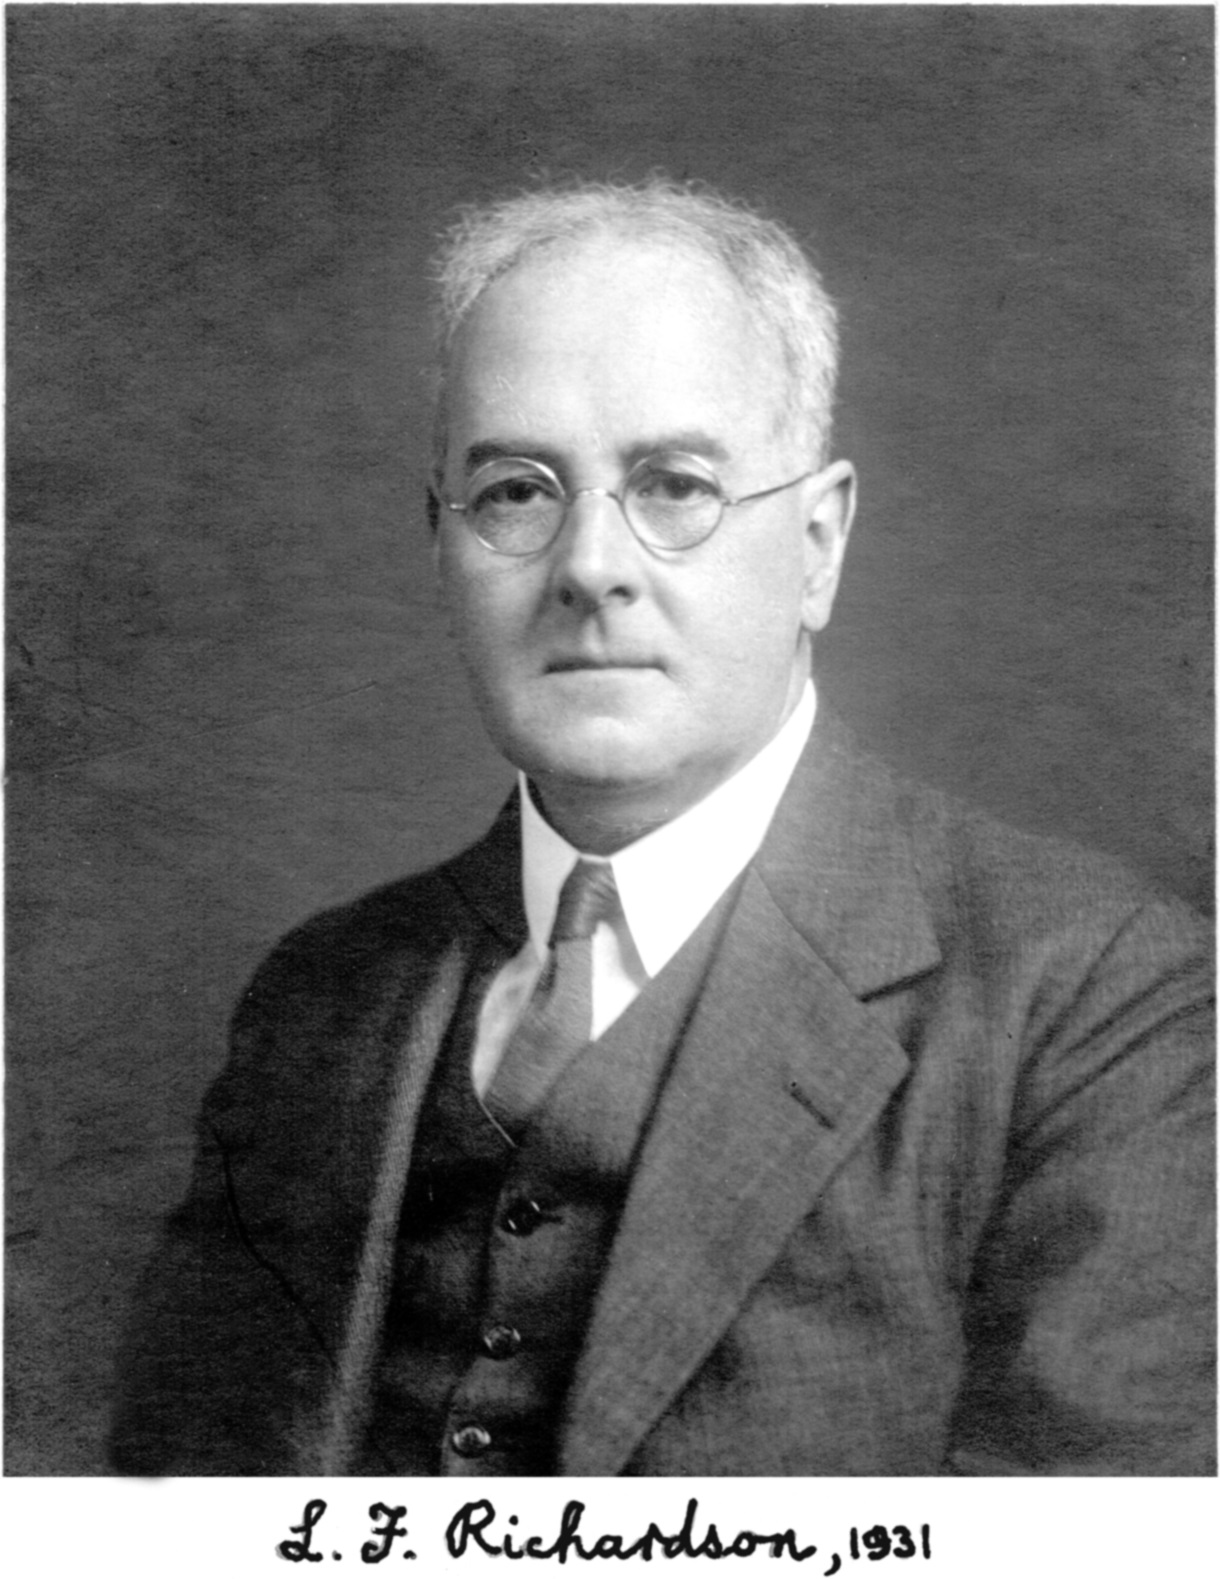
\includegraphics[width=0.4\textwidth]{klima/richardson.jpg}
\caption{Lewis Fry Richardson \cite{klima:biography}
\label{klima:geschichte:richardson}}
\end{figure}

Lewis Fry Richardson (1881-1953) (Abbildung~\ref{klima:geschichte:richardson}) veröffentlichte 1922 seine Arbeit mit dem Titel {\em Weather Prediction by Numerical Process}, in welcher er die erste numerische Wettervorhersage tätigte. Für seine Berechnungen, die er um 1917 durchführte, verwendete er Druck- und Temperatur-Daten verschiedenster Stationen in Europa. Er legte für seine Berechnung ein Gitter über Europa, dieses hatte eine Maschenbreite von 2°89' und eine Maschenlänge von 1°80', und 5 vertikale Layer. Dies entspricht in etwa einer Abmessung von 320km mal 200km je Feld und umfasst insgesamt etwa 150 Punkte, an welchen die Drucktendenz berechnet werden sollte. Er verwendete dabei die horizontalen Impulserhaltungsgleichungen, die ideale Gasgleichung und die Kontinuitätsgleichung \eqref{skript:speziell:kontinuitaetsgleichung} (diese wurde auf Seite \pageref{skript:speziell:kontinuitaetsgleichung} bereits behandelt). Die Vorhersage für 24 Stunden bedeutete einen Rechenaufwand von 3 Monaten. Im Wesentlichen basierte die Berechnung auf einer Unterteilung in die einzelnen Zellen welche jeweils mit 7 Werten befüllt waren. Dies waren der Luftdruck, Temperatur, Dichte, Luftfeuchtigkeit und den Volumenströmen die Richtungen Norden, Osten und Aufwärts.

Die erste Berechnung von Richardson lieferte dann auch ein Resultat, welches einen Druckabfall von 145mbar in 6 Stunden voraussagte. Eine solch grosse Veränderung ist absolut unrealistisch und nicht einmal im Zentrum eines Sturmtiefes möglich. Das Problem war, dass die Daten des Boden-Drucks, welche als Anfangsbedinungen verwendet wurden, Fehler enthielten. Diese Fehler führten dazu, dass sich während der numerischen Prozedur die Werte aufschaukelten und somit zu hohen Drucktendenzen führten. (Eine Berechnung aufgrund der selben Beobachtungsdaten, die jedoch zu Beginn gefiltert werden, führt mit Richardson's Algorithmus zu plausiblen Vorhersagen, 3.2 mbar in 6 Stunden \cite{klima:stocker}).

Dies zeigt exemplarisch wie heikel die Anfangsbedingungen von Wetter- und Klimamodellen sich auf das Ergebnis auswirken können. Jedoch hätten selbst die besten Initialisierungswerte zu einer Instabilität geführt und eine Resultat für grosse Vorhersagezeiten verunmöglicht. Erst durch die Verfügbarkeit erster Computer in den 40er Jahren wurde Richardsons Arbeit zur  Wettervorhersage praktikabel und wurde gegen Ende des 2. Weltkriegs als taktisches Mittel eingesetzt.

\begin{figure}
\centering
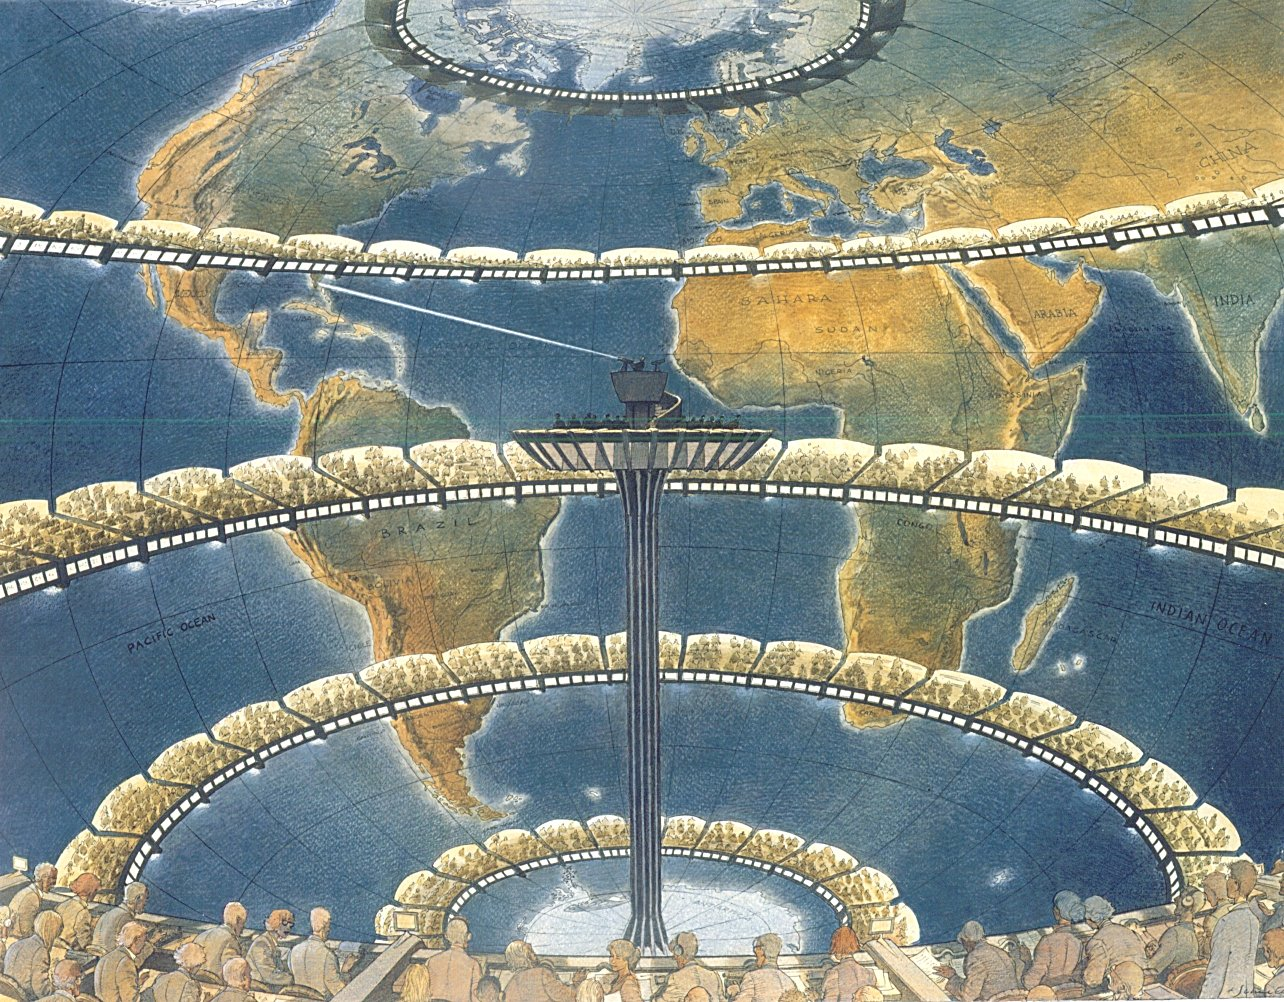
\includegraphics[width=0.9\textwidth]{klima/64000.jpg}
\caption{Interpretation eines Künstlers von Richardsons Vorhersagefabrik \cite{klima:biography}
\label{klima:geschichte:richardson}}
\end{figure}

Richardson äusserte in seiner Arbeit die Idee einer Vorhersagefabrik in welcher er mit 64'000 Rechnern (damit waren damals noch Menschen gemeint), welche gleichzeitig Berechnungen durchführten und zum Weiterrechnen jeweils die Werte ihrer Nachbarzellen übernehmen sollten, das Wetter für den ganzen Planeten berechnen könnte. Diese Idee wurde vom Künstler François Schuiten (Abbildung~\ref{klima:geschichte:richardson}) versinnbildlicht.

Zudem äusserte Richardson einen weiteren Traum:
\begin{quote}
Perhaps some day in the dim future it will be possible to advance the computations faster than the weather advances....
\end{quote}
Von diesem wissen wir, dass es heute nicht nur möglich ist, sondern werden mit jeder neuen Wettervorhersage daran erinnert, dass dies an jedem Tag aufs neue geschieht.

\subsection{Wettervorhersagen in der Schweiz
\label{klima:section:wettervorhersagen}}
\rhead{Wettervorhersagen}

Insgesamt haben wir in der Schweiz sieben private Wetterdienst-Anbieter und den Bundesbetrieb MeteoSchweiz. In diesem Abschnitt wird mehrheitlich auf MeteoSchweiz\index{MeteoSchweiz} und deren Methoden eingegangen, dies weil MeteoSchweiz ihre Methoden im Internet öffentlich einsehbar teilt.

MeteoSchweiz betreibt mit SwissMetNet\index{SwissMetNet} ein eigenes automatisches Messnetz welches ca.160 Station umfässt. Diese liefern alle 10min aktuelle Werte an die zentrale Datenbank der MeteoSchweiz. An einer Standardstation werden kontinuierlich Temperatur, Luftfeuchtigkeit, Luftdruck, Sonneneinstrahlung, Niederschlagsmenge, Windrichtung und -geschwindigkeit erfasst. Doch diese Stationen würden alleine nicht ausreichen, so arbeitet MeteoSchweiz auch mit kantonalen Fachstellen und anderen Institutionen zusammen. Unter anderem werden auch Messwerte von privaten Wetterdienst-Anbietern, welche teilweise eigene Messstationen betreiben, eingekauft. Es handelt sich insgesamt um ca.1500 zertifizierte Messsationen im In- und Ausland.

Zusätzlich werden von MeteoSchweiz Daten zur oberen Atmosphäre erhoben, dies geschieht unter anderem mit Radiosondierungen, hierbei werden in Payerne zweimal täglich Wetterballons gestartet, fünf Wetterradare messen flächendeckend und in Echtzeit den Niederschlag und Gewitter, Windprofiler messen vertikale Windprofile, LIDAR und Ceilometer messen vertikale Feuchtigkeits-, Temperatur- und Aerosolprofile und mit Mikrowellen-Radiometrie wird die  Temperatur und Feuchtigkeit in der Troposphäre gemessen. Des weiteren werden Daten von Wettersatelliten und Ergebnisse aus globalen Wettersimulationen des {\em Europäischen Zentrums für mittelfristige Wettervorhersagen} (ECMWF)\index{Europäisches Zentrum für mittelfristige Wettervorhersagen} für die eigenen Simulationen verwendet. Solch ein grosse Menge an Initialdaten ist unerlässlich, nur dann können von einer Simulation ein verlässliches Resultat erwartet werden. Hinzu kommen die Erfahrungen, welche in zukünftige Simulationen mit einfliessen. \cite{klima:meteoschweiz} 

Der Alpenraum stellt eine besonders hohe Anforderung an Simulationen, so können bei einer zu grossen Maschenweite Täler in einer Simulation nicht korrekt erfasst werden. Ebenso sind Vorhersagen  für Phänomene wie Gewitter, thermische Windsysteme und Föhn besonders schwierig. MeteoSchweiz setzt bei Simulationen auf das numerische Wettervorhersagemodell COSMO-CLM (COSMO Climate Limited-area Model) welches in verschiedenen Varianten betrieben wird. Für enge Täler, wie beispielsweise das Lauterbrunnental, ist genauste Auflösung von 1.1 km immer noch zu grob als dass eine genaue Vorhersage jeglicher Parameter gemacht werden kann.
Im Allgemeinen werden folgende Parameter zur Beschreibung des Wetters bestimmt: Temperatur, Luftfeuchtigkeit, Gesamtniederschlag (Regen und Schnee), Wind, Luftdruck und Geopotential, Bewölkung, Strahlung, Verdunstung und Schneefallgrenze.

\begin{figure}
\centering
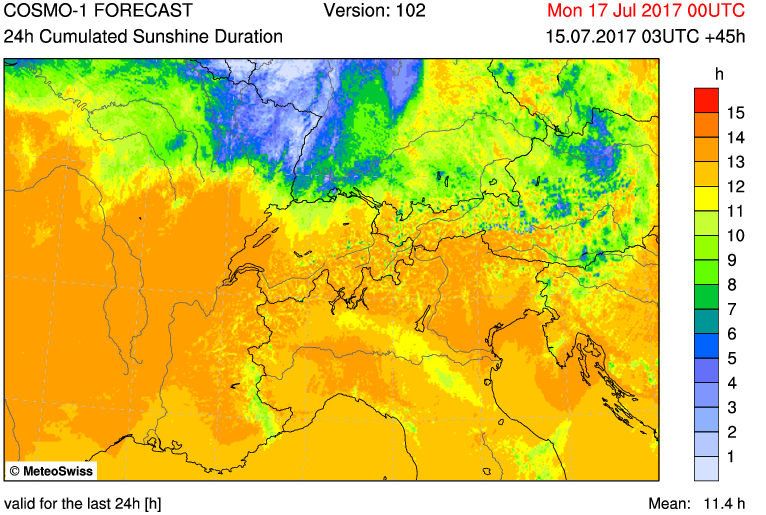
\includegraphics[width=0.9\textwidth]{klima/cosmo1.png}
\caption{COSMO-1 24-Stunden-Summe Vorhersage für Sonnenschein am 15.07.2017 \cite{klima:meteoschweiz}
\label{klima:wettervorhersagen:cosmo}}
\end{figure}

\begin{itemize}
\item COSMO-1: $1158 \times 774$ Gitterpunkte; Maschenweite 1.1 km (0°01'); 80 vertikale Schichten; gesamter Alpenbogen mit der Schweiz im Zentrum; Zeitschrittweite 10 Sekunden; Voraussagen bis 45h, 8mal täglich; Geeignet für bessere Vorhersagen, insbesondere Gewitter, thermische Windsysteme und Föhn \cite{klima:meteoschweiz}
% Funfact, CFL = 10s / 1100m * 343 m/s = 3.12 Es scheint das Wettervorhersagen mit COSMO bereits bei einer Courant-Friedrich-Levi-Zahl von ca. 3.12 verlässlich sind. Üblich ist in numerischen Simulationen ein Wert von 1, dies würde jedoch einen 3mal höheren Rechenaufwand bedeuten.
\item COSMO-7: $393 \times 338$ Gitterpunkte; Maschenweite 6.6 km (0° 06'); 60 vertikale Schichten; ganz West- und Mitteleuropa; Voraussagen bis 72h, 3mal täglich \cite{klima:meteoschweiz} 
\item COSMO-E: $582 \times 390$ Gitterpunkte; Maschenweite 2.2 km (0° 02'); 60 vertikale Schichten; gesamter Alpenbogen mit der Schweiz im Zentrum; 21 Ensemble-Rechnungen mit leicht variierenden Initialwerten mit gleich wahrscheinlichen Vorhersagen; Geeignet für Wahrscheinlichkeitsvorhersagen von extremen Ereignissen wie Stürme oder Starkniederschläge \cite{klima:meteoschweiz} 
\end{itemize}

\subsection{Klimavorhersagen
\label{klima:subsection:entstehung}}
\rhead{Klimavorhersagen}
Die {\em Weltorganisation für Meteorologie} (WMO)\index{Weltorganisation für Meteorologie} definiert das Klima als die Statistik des Wetters über einen Zeitraum, der lang genug ist, um diese statistischen Eigenschaften auch bestimmen zu können. Während das Wetter den physikalischen Zustand der Atmosphäre zu einem bestimmten Zeitpunkt an einem bestimmten Ort beschreibt, ist Klima erst dann richtig gekennzeichnet, wenn die Wahrscheinlichkeit für Abweichungen vom Mittelwert angegeben werden kann, also auch Extremwerte Teil der Statistik sind. Zur Beschreibung des Klimas wird in der Regel eine Zeitspanne von 30 Jahren als Bezugszeitraum herangezogen. Die übliche Einteilung in Klimazonen folgt überwiegend dem Jahresgang der Temperatur und des Niederschlags \cite{klima:maxplanck}.

Die ersten Klimamodellen wurden bereits in den 1960er Jahren genutzt, es handelte sich im Wesentlichen um einfache Energiebilanzmodelle von Strahlung und Wärme. Eine Modellierung der Atmosphäre wäre zu dieser Zeit aufgrund der fehlenden Rechenkapazität nicht möglich gewesen. Jedoch konnten auch mit diesen einfachen Modellen bereits Aussagen zum Temperaturanstieg aufgrund des CO$_2$-Anstiegs getätigt werden. In den 1970er Jahren wurde es, dank der steigenden Rechenkapazität, erstmals möglich, Wettervorhersagemodelle für die Klimaforschung einzusetzen. Die Verwendung etablierter Programme bringt einige Vorteile mit sich, so müssen diese nicht von Grund auf neu entwickelt werden. Ein Nachteil liegt jedoch in den grossen Rechenleistungen welche, wie beim Wetter, für zuverlässige Aussagen benötigt werden.
 
Es gibt viele verschiedene Parameter welche einen Einfluss auf das Klima haben, so gehören dazu  allgemeine Dinge wie Sonneneinstrahlung, Zusammensetzung der Atmosphäre und Oberflächenbeschaffenheit (Wasser, Wüste, Wälder, Wiese, etc.). Seit der Industrialisierung beeinflusst der Mensch die Luftzusammensetzung mit dem vermehrten Ausstoss von CO$_2$, jedoch ist dies nicht die einzige Einflussnahme des Menschen, so gibt es viele Dinge, welche sich direkt oder indirekt auf das Klima auswirken. Als Beispiel setzt die Abholzungen von Wäldern zusätzlich CO$_2$ frei. Wälder sind jedoch auch hervorragende Wasserspeicher, dieses Wasser verdunstet und ist oft für Regen in trockeneren Gebieten verantwortlich. Sind die Wälder nicht mehr vorhanden, können andere Regionen plötzlich mit Trockenheit zu kämpfen haben.

Das Klima ist ein heikles System, so weist es verschiedenste Rückkopplungseffekte und Kipppunkte auf. So beschreibt die Eis-Albedo-Rückkopplung den Effekt der Rückstrahlung der Sonnenstrahlen auf Eis, wie zum Beispiel in der Arktis. Sollte dieses Eis verschwinden und dafür das arktische Meer die Oberfläche bilden wird die Sonnenstrahlung zu einem grossen Teil absorbiert und nicht mehr zurück in den Weltraum gestrahlt. Hierbei wandelt sich die Strahlung in Wärme um und sorgt für eine noch schnellere Erwärmung unseres Klimasystems. Ein Kipppunkt bildet das Auftauen der Permafrostböden, beim Auftauen wird dass darin vorhandene Methan, ein Treibhausgas, freigesetzt, gelangt in die Atmosphäre und treibt damit die Klimaerwärmung zusätzlich an, dieser Vorgang ist irreversible.

\section{Spektrale Methoden
\label{klima:section:spektrale}}
\rhead{Beispiel: Wärmeleitung}
Im Gegensatz zur klassischen Strömungsmechanik, welche mit Differenzmethoden arbeiten, wählen die spektralen Methoden einen globalen Ansatz. Hierbei wird das Ergebnis in den Spektralbereich transformiert und ist keine physikalische Grösse wie Druck oder Temperatur.

\subsection{Beispiel Wärmeleitungsgleichung}
Wie im Abschnitt \ref{klima:subsection:entstehung} \nameref{klima:subsection:entstehung} aufgezeigt handelt es sich bei unserer Atmosphäre um ein hochkomplexes System, deren Eigenheiten bis zum heutigen Zeitpunkt noch nicht restlos verstanden sind und deshalb immer noch Teil der Forschung ist. Ein komplexes System wie das Klima kann somit unmöglich in einigen wenigen Zeilen mathematisch hergeleitet und beschrieben werden. Wir schränken uns aus diesem Grund bei den Beispielen auf ein einziges Problem, die Wärmeleitung, ein. Die Problemstellung ist einfach zu verstehen, veranschaulicht jedoch die mathematischen Schwierigkeiten und deren Komplexität sehr gut.

Für die Aufgaben wird die allgemeine Wärmeleitungsgleichung\index{Wärmeleitung}
\begin{align}
\frac{\partial T}{\partial t} = \Delta T
\label{klima:bsp:pdgl}
\end{align}
benötigt.

\subsection{Lösung der Wärmeleitungsgleichung mit Differenzenmethoden}
Damit wir die Komplexität eines herkömmlichen Modells, welches mit Differenzen arbeitet, mit dem der spektralen Methoden vergleichen können, schauen wir dies an einem vereinfachten Beispiel an. Wir betrachten die Wärmeleitung eines Stabes.
Der Laplace-Operator ist bei einem eindimensionalen Problem gerade die zweite Ableitung der Funktion, somit ergibt sich aus der Allgemeinen, die spezielle Wärmeleitungsgleichung.\index{Wärmeleitung}
\begin{align}
\frac{\partial T}{\partial t} = \Delta T \rightarrow \frac{\partial T}{\partial t}=\dfrac{\partial^2 T}{\partial x^2}
\end{align}
Es werden die dazugehörigen Differenzenquotienten\index{Differenzenquotient}
\begin{align}
\frac{\partial T}{\partial t}
&\rightarrow
\frac{\Delta T}{\Delta t}=
\frac{T(t+\Delta t,x)-T(t,x)}{\Delta t}
\\
\frac{\partial^2 T}{\partial x^2}
&\rightarrow
\frac{T(t,x+\Delta x)-2T(t,x)+T(t,x-\Delta x)}{\Delta x^2}
\end{align}
benötigt. Mit diesen lässt sich nun die Gleichung
\begin{align}
\frac{T(t+\Delta t,x)-T(t,x)}{\Delta t}
=
\frac{T(t,x+\Delta x)-2T(t,x)+T(t,x-\Delta x)}{\Delta x^2}
\end{align}
erstellen. Nach $T(t+\Delta t,x)$ umgeformt ergibt sich die Gleichung
\begin{align}
T(t+\Delta t,x)
=
T(t,x)+\Delta t \frac{T(t,x+\Delta x)-2T(t,x)+T(t,x-\Delta x)}{\Delta x^2},
\label{klima:bsp:diff}
\end{align}
diese wird für die numerische Berechnung benötigt wird.

Mit der Gleichung \eqref{klima:bsp:diff} wird die Temperatur des nächsten Zeitschritt $T(t+\Delta t,x)$ berechnet. Dies ist ebenso in der Abbildung~\ref{klima:wettervorhersagen:diff} illustriert. Wir können daher sagen, möchte man die Temperaturänderung eines Punktes zu seinem vorherigen Zustand wissen, so benötigt man dessen eigenen Wert $T(t,x)$ und die Werte der beiden benachbarten Punkte $T(t,x+\Delta x)$ und $T(t,x-\Delta x)$. Daraus lässt sich folgern, dass sich Einflüsse in der Simulation maximal mit $\frac{\Delta x}{\Delta t}$ ausbreiten können. Sollte eine Problemstellung bearbeitet werden in welcher sich etwas schneller ausbreitet, als dies in der Simulation geschehen kann, führt dies zu Fehlern in der Auswertung. Möchte man das Problem beheben, so kann man entweder die Punktabstände $\Delta x$ erhöhen oder die Zeitschritte $\Delta t$ verkleinern, zweites führt jedoch zu erhöhtem Rechenaufwand. Es ist festzuhalten dass Modelle, welche auf den Differenzmethoden beruhen, eine endliche Ausbreitungsgeschwindigkeit haben.

\begin{figure}
\centering
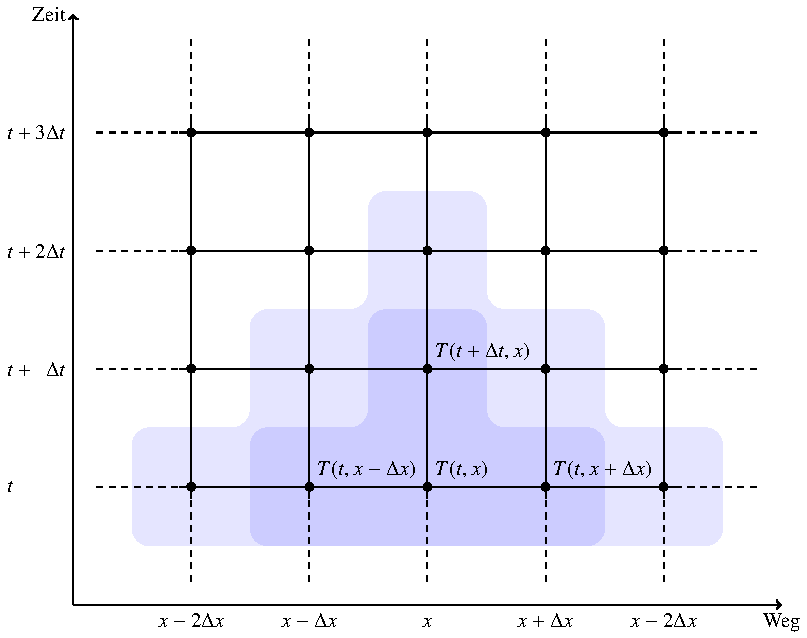
\includegraphics[width=0.9\textwidth]{klima/differenzen.pdf}
\caption{
\label{klima:wettervorhersagen:diff}}
\end{figure}

Möchte man mit den Differenzmethoden eine Simulation durchführen, bedingt dies, dass diese Berechnungen für jeden Punkt zu jedem Zeitschritt gemacht werden muss. Dies führt dazu, dass Simulationen sehr rechenintensiv sind.

\subsection{Lösung der Wärmeleitungsgleichung mit spektralen Methoden}
Für die spektralen Methoden werden im Wesentlichen die Wärmeleitungsgleichung \eqref{klima:bsp:pdgl}
und eine Ansatzfunktion, wie die Fourier-Reihen, benötigt.\index{Wärmeleitung}

\subsubsection{Lösung der Wärmeleitungsgleichung}
In diesem Abschnitt soll mithilfe der Fourier-Theorie die Wärmeleitungsgleichung auf einer Kugel gelöst werden. Eine Übungsaufgabe in welcher mithilfe der Fourier-Theorie die  Wärmeleitungsgleichung auf einem Kreis gelöst wurde, befindet sich am Ende des Kapitels \ref{skript:chapter:kugelfunktionen} \nameref{skript:chapter:kugelfunktionen} auf der Seite \pageref{skript:1101:pdgl}.

Für die Konstruktion unseres Modells wird die Fourier-Reihe auf der Kugel benötigt:
\begin{align}
T(\vartheta ,\varphi ,t)
=
a^0_0(t) + \sum_{l=1}^\infty\sum_{m=0}^l \bigl( a^m_l(t)\,Y^m_l(\vartheta ,\varphi)+b^m_l(t)\,Z^m_l(\vartheta ,\varphi) \bigr).
\label{klima:equation:fourier}
\end{align}
Deren Herleitung wird im Abschnitt \ref{skript:chapter:kugelfunktionen} \nameref{skript:chapter:kugelfunktionen} behandelt.

Die Gleichung \eqref{klima:equation:fourier} stellt im Wesentlichen das Modell dar, $\vartheta$ steht dabei für den Längengrad und $\varphi$ für den Breitengrad. Zur Berechnung der Spektralkoeffizienten\index{Spektralkoeffizient} $a^m_l(t)$ und $b^m_l(t)$ wird die folgende Eigenschaft der Kugelfunktion für den Laplace-Operator benötigt:
\begin{align}
\Delta \,Y^m_l=-l(l+1)\,\,Y^m_l.
\label{klima:equation:laplace}
\end{align}

Als erstes stellen wir die gewöhnliche Differentialgleichung auf, dazu muss die Fourier-Reihe~\eqref{klima:equation:fourier} für $T(\vartheta ,\varphi ,t)$ in die Differentialgleichung~\eqref{klima:bsp:pdgl} eingesetzt werden.
Dazu berechnen wir die Ableitungen nach $t$ und setzen die Gleichung \eqref{klima:equation:laplace} ein.
\begin{align*}
\frac{\partial T(\vartheta ,\varphi ,t)}{\partial t} &=
\dot{a}^0_0(t)+\sum_{l=1}^\infty\sum_{m=0}^l \bigl( \dot{a}^m_l(t)\,Y^m_l(\vartheta ,\varphi)+\dot{b}^m_l(t)\,Z^m_l(\vartheta ,\varphi)\bigr)
\\
\Delta T(\vartheta ,\varphi ,t) &=
- \sum_{l=1}^\infty\sum_{m=0}^l \bigl( a^m_l(t)\,l(l+1)\,Y^m_l(\vartheta ,\varphi)+b^m_l(t)\,l(l+1)Z^m_l(\vartheta ,\varphi)\bigr)
\end{align*}
Die Differentialgleichung verlangt, dass diese beiden Terme übereinstimmen, also folgen die gewöhnlichen Differentialgleichungen
\begin{align*}
\dot a^0_0(t)&= 0
\\
\dot a^m_l(t)&=-l(l+1)a^m_l(t)&
\dot b^m_l(t)&=-l(l+1)b^m_l(t).
\end{align*}
Man beachte, dass die erste Gleichung als Spezialfall in der ersten
Gleichung der zweiten Zeile enthalten ist.
\begin{align*}
a^0_0(t)&=\text{const.}
\\
a^m_l(t) &=Ae^{-l(l+1)t}&
b^m_l(t) &=Be^{-l(l+1)t}
\end{align*}

Möchte man die Kugelfunktionen $Y^m_l$ und $Z^m_l$ berechnen, so kann dies mit der Gleichung \eqref{skript:kugelfunktione:Y} auf der Seite \pageref{skript:kugelfunktione:Y} gemacht werden. Dies ist jedoch für das Verständnis nicht notwendig, so beschreiben diese Funktionen lediglich den Unterschied zum Mittelwert $a^0_0(t)$, in diesem Falle der globalen Mitteltemperatur. Wie sich der Unterschied entwickeln wird ist durch die $a^m_l(t)$ und $b^m_l(t)$ definiert.

\subsubsection{Konstanter Erwärmungsterm
\label{klima:subsubsection:erwaermungsterm}}
\index{Erwärmungsterm}
Wie wir im vorherigen Abschnitt gesehen haben ist die Lösung für die globale Mitteltemperatur $a^0_0(t)=\text{const.}$, wenn dies wirklich so wäre, gäbe es keine Klimaerwärmung. Da uns bekannt ist, dass diese existiert, muss die Differenzialgleichung umgeschrieben werden.
\begin{align}
\dot a^0_0(t)=E(t)
\end{align}
Es ergibt sich daraus neu die Gleichung
\begin{align}
a^0_0(t)=T_0 \cdot e^{E(t)\cdot t}.
\end{align}
$T_0$ steht dabei für die globale Temperatur. In den meisten Klimamodellen ist dies die globale Temperatur vor der industriellen Zeit dar (ca. 1850). (Genauso verhält sich dies in der Abbildung~\ref{klima:einleitung:nasa}.) Das bedeutet dass der CO$_2$ Anstieg Bestandteil von $E(t)$ sein muss. Dies könnte wie folgt aussehen:
\begin{align}
E(t)=\delta_{\text{CO}_2}+\delta_{\text{Methan}}+\delta_{\text{Wasserdampf}}+...
\end{align}
Mit dem $E(t)$ kann nun der Anstieg der globalen Mitteltemperatur berechnet werden.

\subsubsection{Temperaturunterschiede zwischen Nord- und Südhalbkugel
\label{klima:subsubsection:halbkugel}}
\index{Temperaturunterschiede zwischen Nord- und Südhalbkugel}
Möchte man ein kleines Klimamodell definieren, so muss  $m$ und $l$ festgelegt werden, diese ist Abhängig von der Komplexität welche erreicht werden möchte. Da wir in unserem Beispiel diese klein halten wollen, entscheiden wir uns für $l=1$ und $m=0$, dieses Beispiel gliedert unseren Planeten in der Modellierung in Nord- und Südhalbkugel auf. Mit höheren $m$ und $l$ würden wir unseren Planeten in weitere Bereiche gliedern und die Modellierung komplexer gestalten, jedoch möchten wir genau dies nicht.
\begin{align*}
a^0_0(t)&=E(t)+T_0
\\
a^0_1(t) &=Ae^{-2t}&
b^0_1(t) &=Be^{-2t}
\end{align*}
Bei der speziellen Situation von $m=0$ ergibt sich
\begin{align*}
Y^0_l=Z^0_l.
\end{align*}
Damit und aus der Gleichung \eqref{klima:equation:fourier} entsteht nun neu
\begin{align}
T(\vartheta ,\varphi ,t)
=
\underbrace{a^0_0(t)}_{\text{Global}} + \underbrace{\bigl( a^0_1(t)+b^0_1(t) \bigr)}_{\text{Spektral-Koeffizienten}} \cdot \underbrace{Y^0_1(\vartheta ,\varphi)}_{\text{Kugelfunktion}}.
\end{align}
Ein Grossteil der CO$_2$ Emissionen, ein Treibhausgas, geschehen auf der Nordhalbkugel. Dies hat einen direkten Einfluss darauf, dass sich das Klima auf der Nordhalbkugel wegen der grösseren CO$_2$ Konzentrationen mehr erwärmt, dies führt zu einem Rückkopplungseffekt. Somit muss die Funktion $\dot a^0_1(t)$ modifiziert werden,
\begin{align*}
\dot a^0_1(t) &= 2a_1^0+\delta_{\text{CO}_2} &
a_1^0 &= Ae^{-2t-\delta_{\text{CO}_2}(t)}
\end{align*}
das $\delta_{CO_2}(t)$ stellt dabei die zusätzliche Erwärmung dar. Ebenso kann man die unterschiedlichen Einflüsse der Jahreszeiten modellieren. So ist die Sonneneinstrahlung unter anderem von der Jahreszeit abhängig, dies könnte in der Modellierung folgendermassen ausschauen:
\begin{align*}
\dot a_1^0(t) &= 2a_1^0 \cos(\gamma_{\text{Jahr}}(t)) &
\dot b_1^0(t) &= 2a_1^0 \sin(\gamma_{\text{Jahr}}(t))
\\
a_1^0 &= Ae^{-2t \cos(\gamma_{\text{Jahr}}(t)} &
b_1^0 &= Be^{-2t \sin(\gamma_{\text{Jahr}}(t)}
\end{align*}

\subsection{Anwendung der spektralen Methoden}
\rhead{Anwendung}
In den vorherigen Abschnitten wurden Beispiele für die Differenzenmethode und die spektralen Methoden anhand der Wärmleitungsgleichung gezeigt. Dabei lassen sich bereits die wesentlichen Vorteile der spektralen Methoden erkennen, so ist diese nicht auf Zeitschritte angewiesen, beschreiben nicht nur einzelne Punkte sondern ganze Gebiete und zusätzliche Einflussfaktoren können relativ einfach modelliert werden. Sie eignen sich für Funktionen mit einer hohen Glattheit. Ein grosser Nachteil liegt in ihrem globalen Ansatz, möchte man die Auflösung eines bestimmten Gebietes erhöhen, muss dies global geschehen. Dies lässt die spektralen Methoden für kleinräumige Probleme, wie das Wetter, weniger nützlich erscheinen. Es ist somit ein Vorteil der Differenzenmethode Gebiete genauer darstellen zu können, da dies für Klimamodelle jedoch nicht benötigt wird, eigenen sich spektrale Modelle hervorragend für solche.
 
Die spektralen Methoden\index{spektrale Methoden} werden heute bereits in einigen Modellen eingesetzt, so beispielsweise beim {\em Integrated Forecast System} (IFS)\index{Integrated Forecast System} einem globalen Wettervorhersage-Modell des {\em Europäischen Zentrums für mittelfristige Wettervorhersagen} (ECMWF)\index{Europäisches Zentrum für mittelfristige Wettervorhersagen}. So wurde dort bereits im April 1983 das erste spektrale Modell in Betrieb genommen.

Heute werden die spektralen Modelle im IFS in Zusammenarbeit mit Differenzmethoden eingesetzt. So wird mit der spektralen Methode der horizontale Wind, die virtuelle Temperatur und der Oberflächendruck berechnet. Die Werte werden hierbei bei jedem Zeitschritt für die Differenzenmethode transformiert und für den nächsten Zeitschritt rücktransformiert \cite{klima:ecmwf}.


\printbibliography[heading=subbibliography]
\end{refsection}
